\chapter{Atmospheric Pressure}

The air you breathe is a blend of gases:
\begin{enumerate}
\item 78\% nitrogen in the form of $N_2$
\item 21\% oxygen in the form $O_2$
\item 1\% other gases (mostly argon)
\end{enumerate}

If you fill a balloon with helium ($He$),  the helium will push against the interior of the balloon with some pressure.   
The pressure is the same at every point in the interior of the balloon.  Pressure,  then,  is force spread over some area.   
Force is commonly measured in newtons.   Pressure is measured in \newterm{pascals}.  A pascal is 1 newton per square meter.

We don't usually think about it,  but the air outside the balloon is also pushing against the exterior of the balloon.  
We call this \newterm{barometric pressure} or \newterm{atmospheric pressure} and it is caused by gravity pulling on the gas molecules above the balloon.
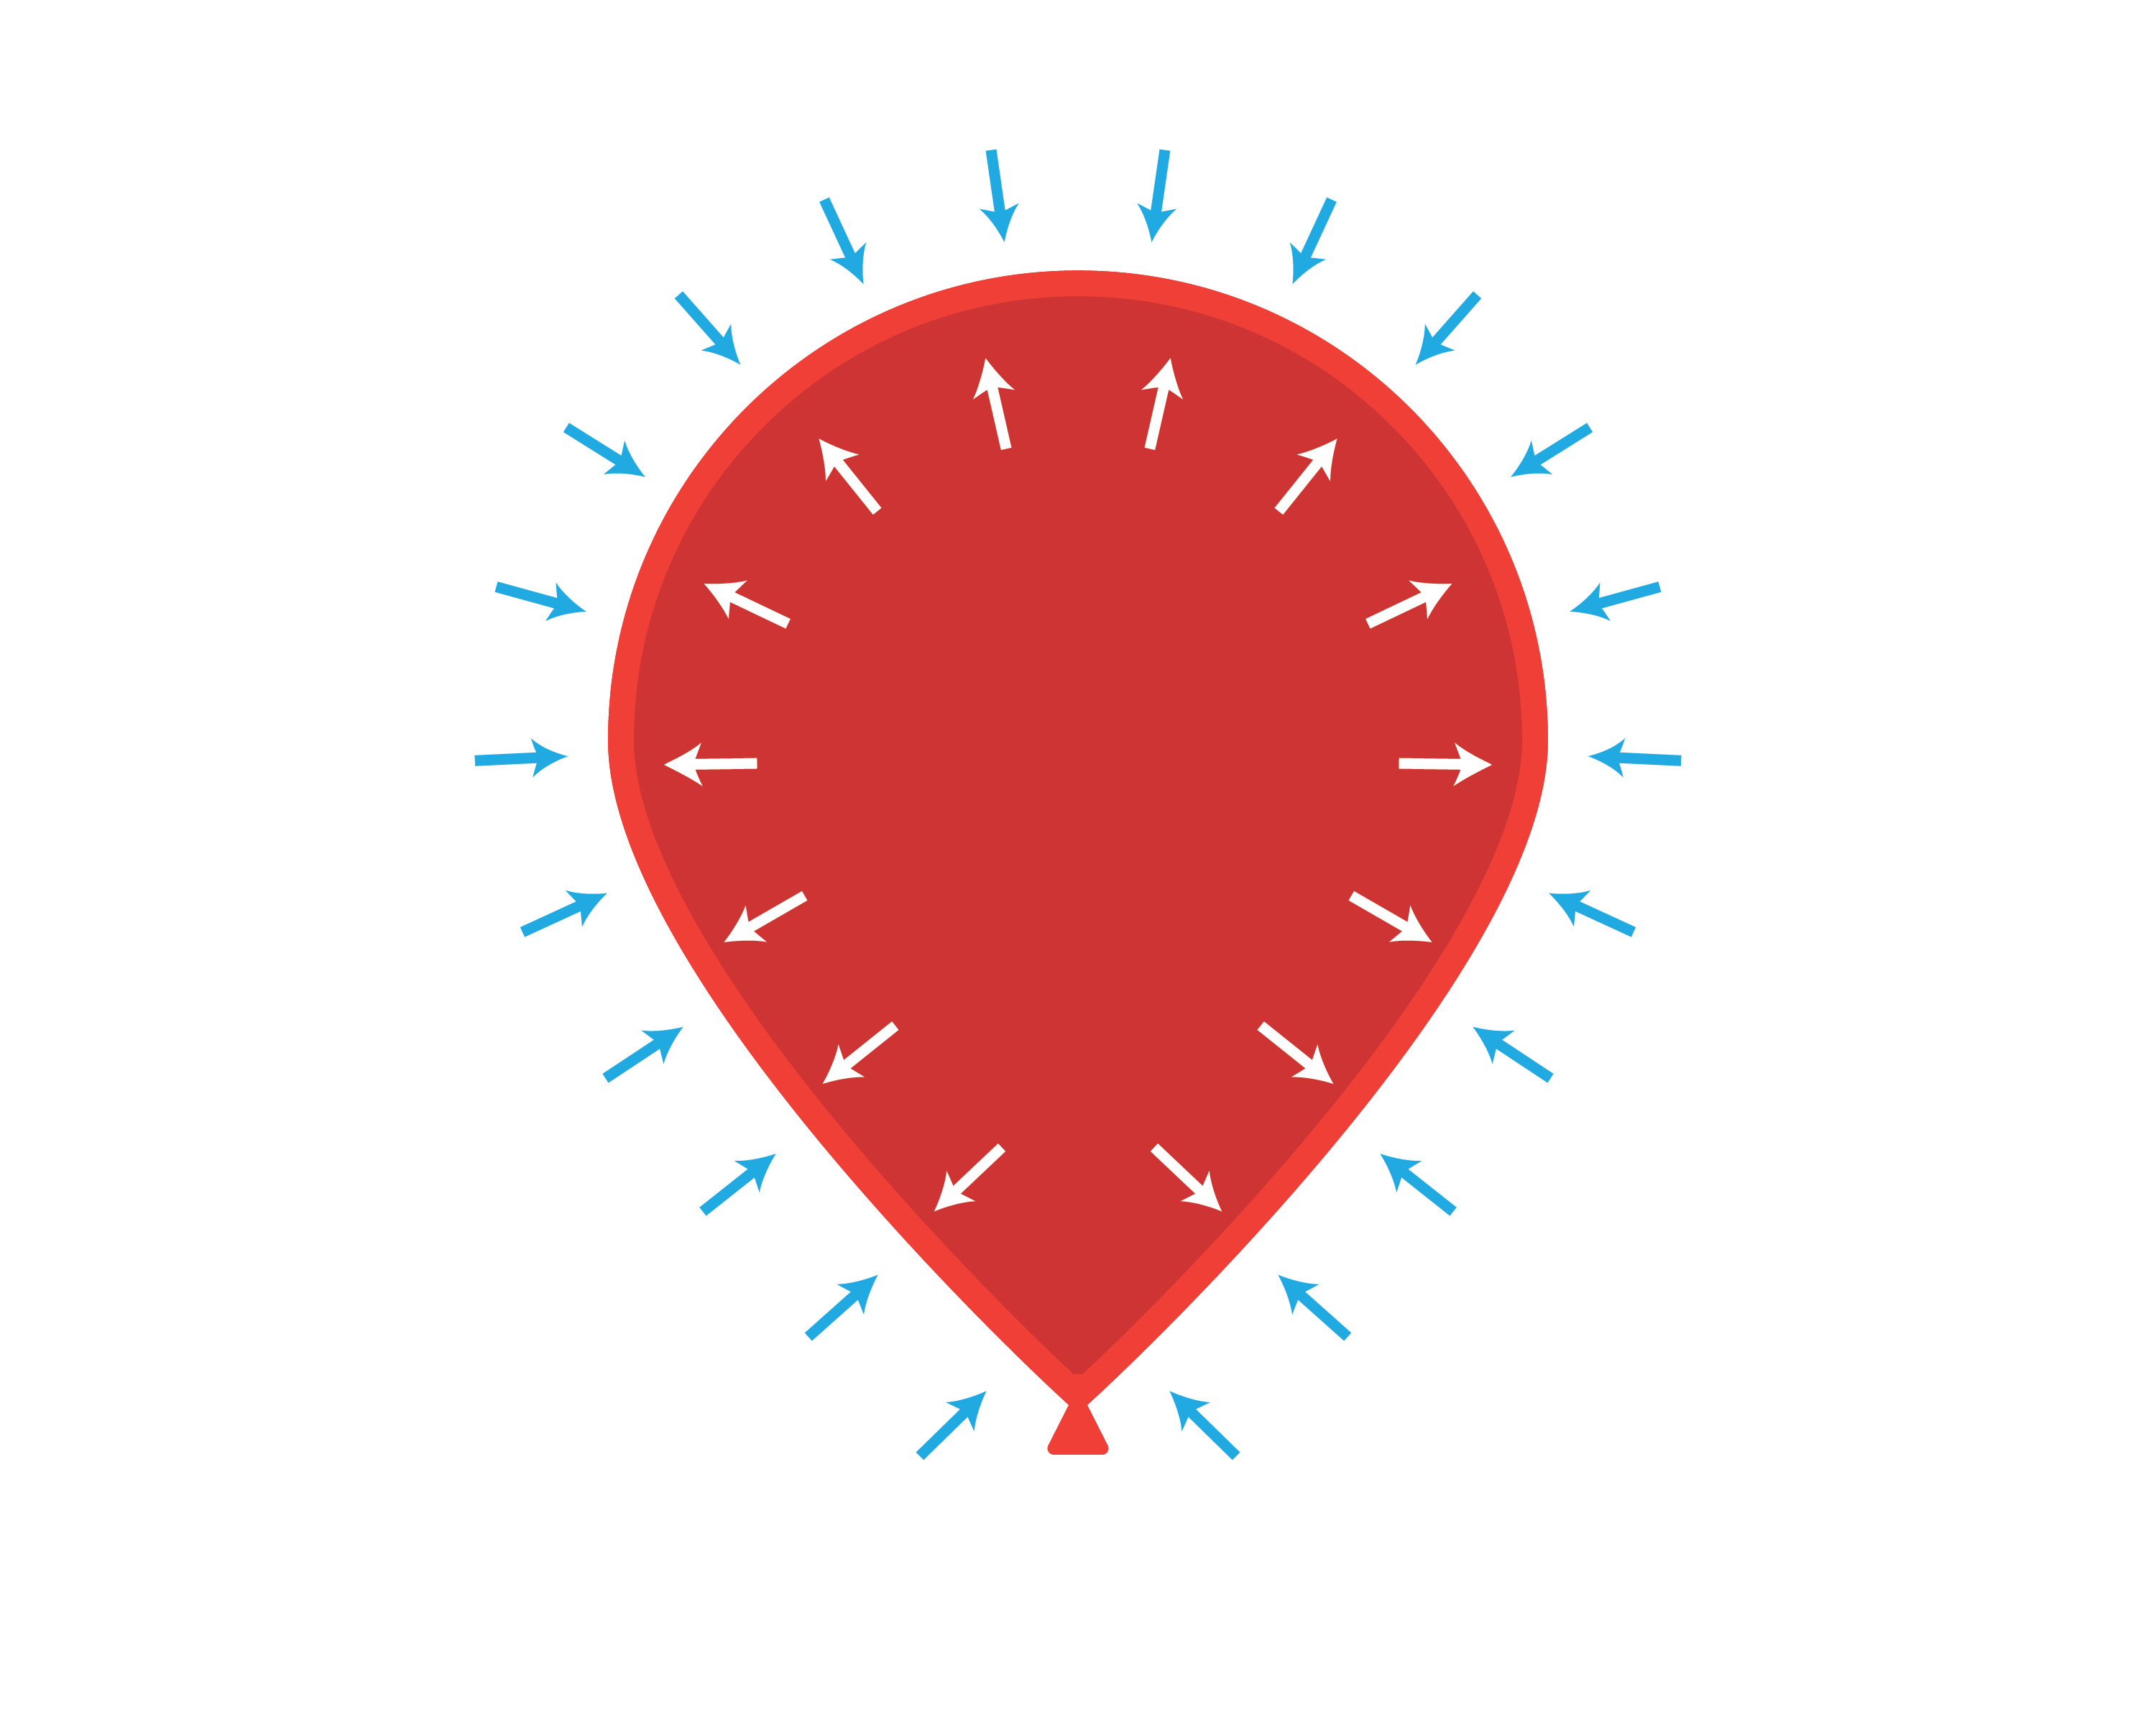
\includegraphics[width=\textwidth]{balloon.png}


Imagine a square meter on the ground at sea level.  Now imagine the column of air above it -- reaching all the way to the top of the atmosphere.

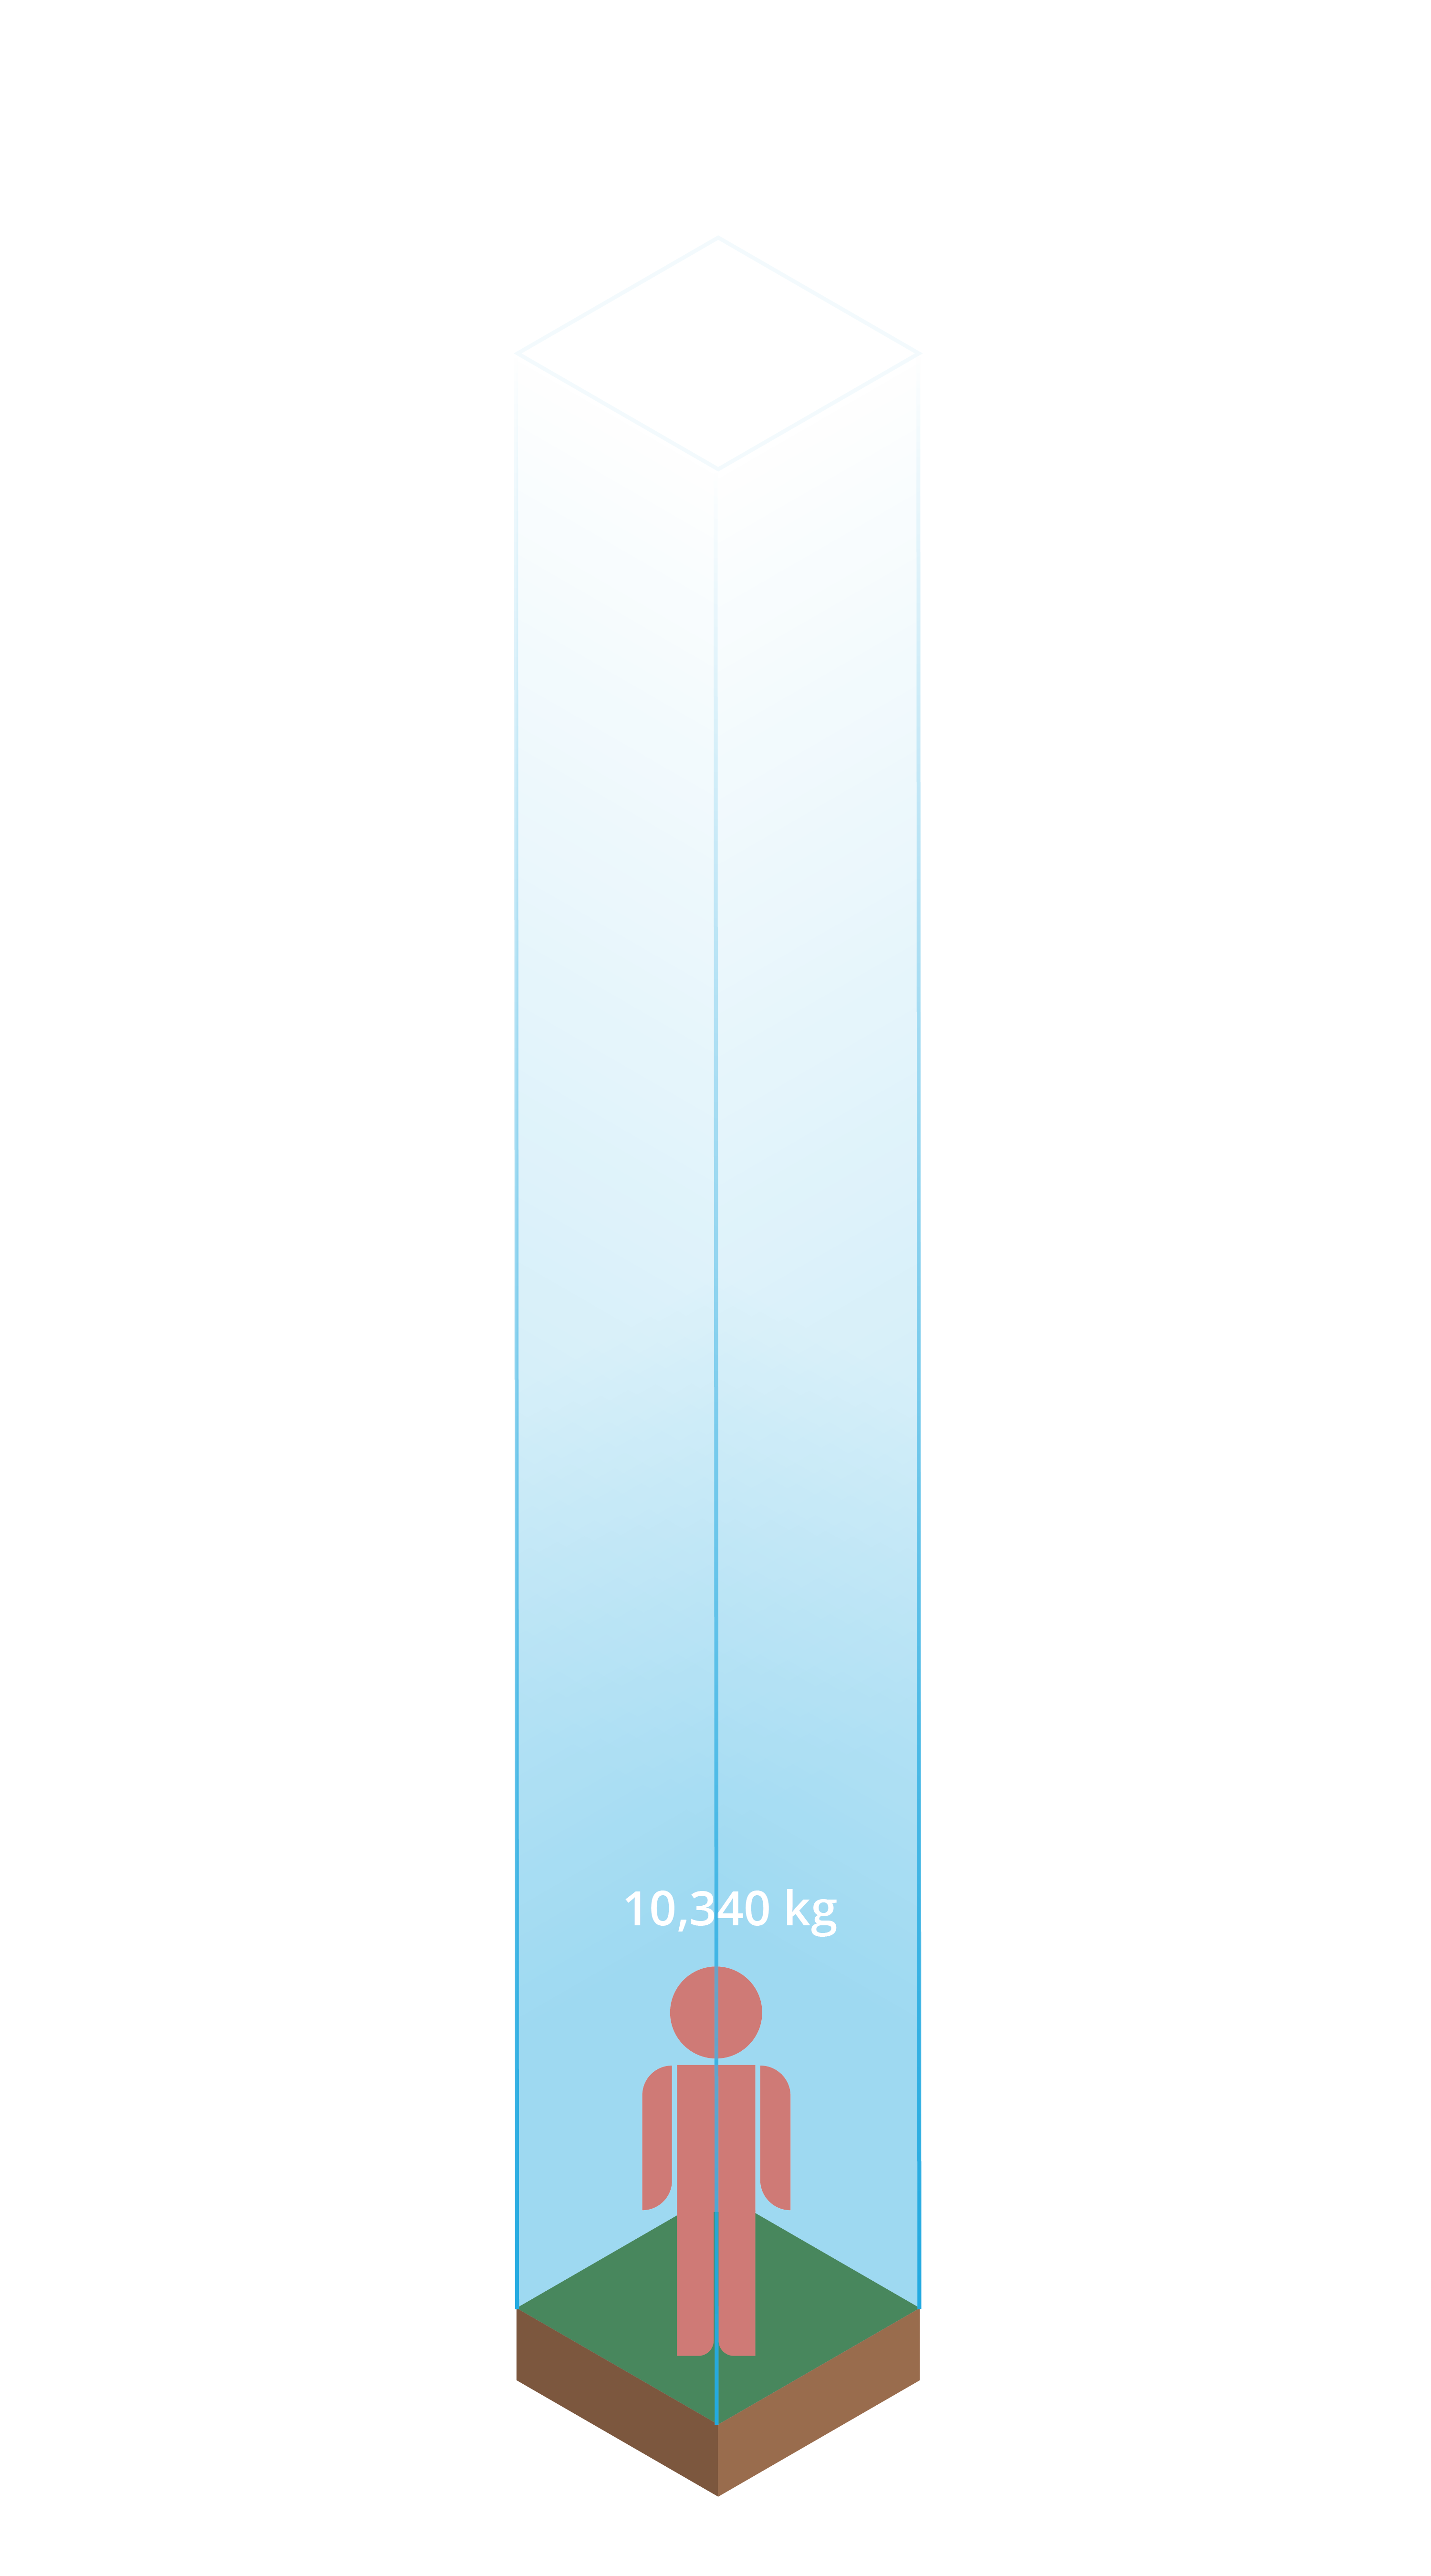
\includegraphics[width=\textwidth]{aircolumn.png}

The air inside that column has a mass of about 10,340 kg.  One kilogram on the earth experiences a gravitational force of 9.8 N.   
So the atmospheric pressure all around you is about 101,332 pascals.  
When dealing with such large numbers, we often use kilopascals.  
We'd say the barometric pressure at sea level is about 101.3 kPa.

That's a lot of pressure!  Why doesn't your ribcage collapse crushing your lungs?  The air \emph{inside} your lungs is the same 
pressure as the air push on the outside of your rib cage.  

And thus we live pretty much oblivious to this huge force that is all around us, but you can see it sometimes.  
For example, if you suck the air out of a plastic bottle,   the bottle will be crushed by the barometric pressure.

\section{Altitude and Atmospheric Pressure}

If you let go of the balloon, as it rises through this column there will be less and less air mass above it, and thus less and less atmospheric pressure on the outside of the balloon. 

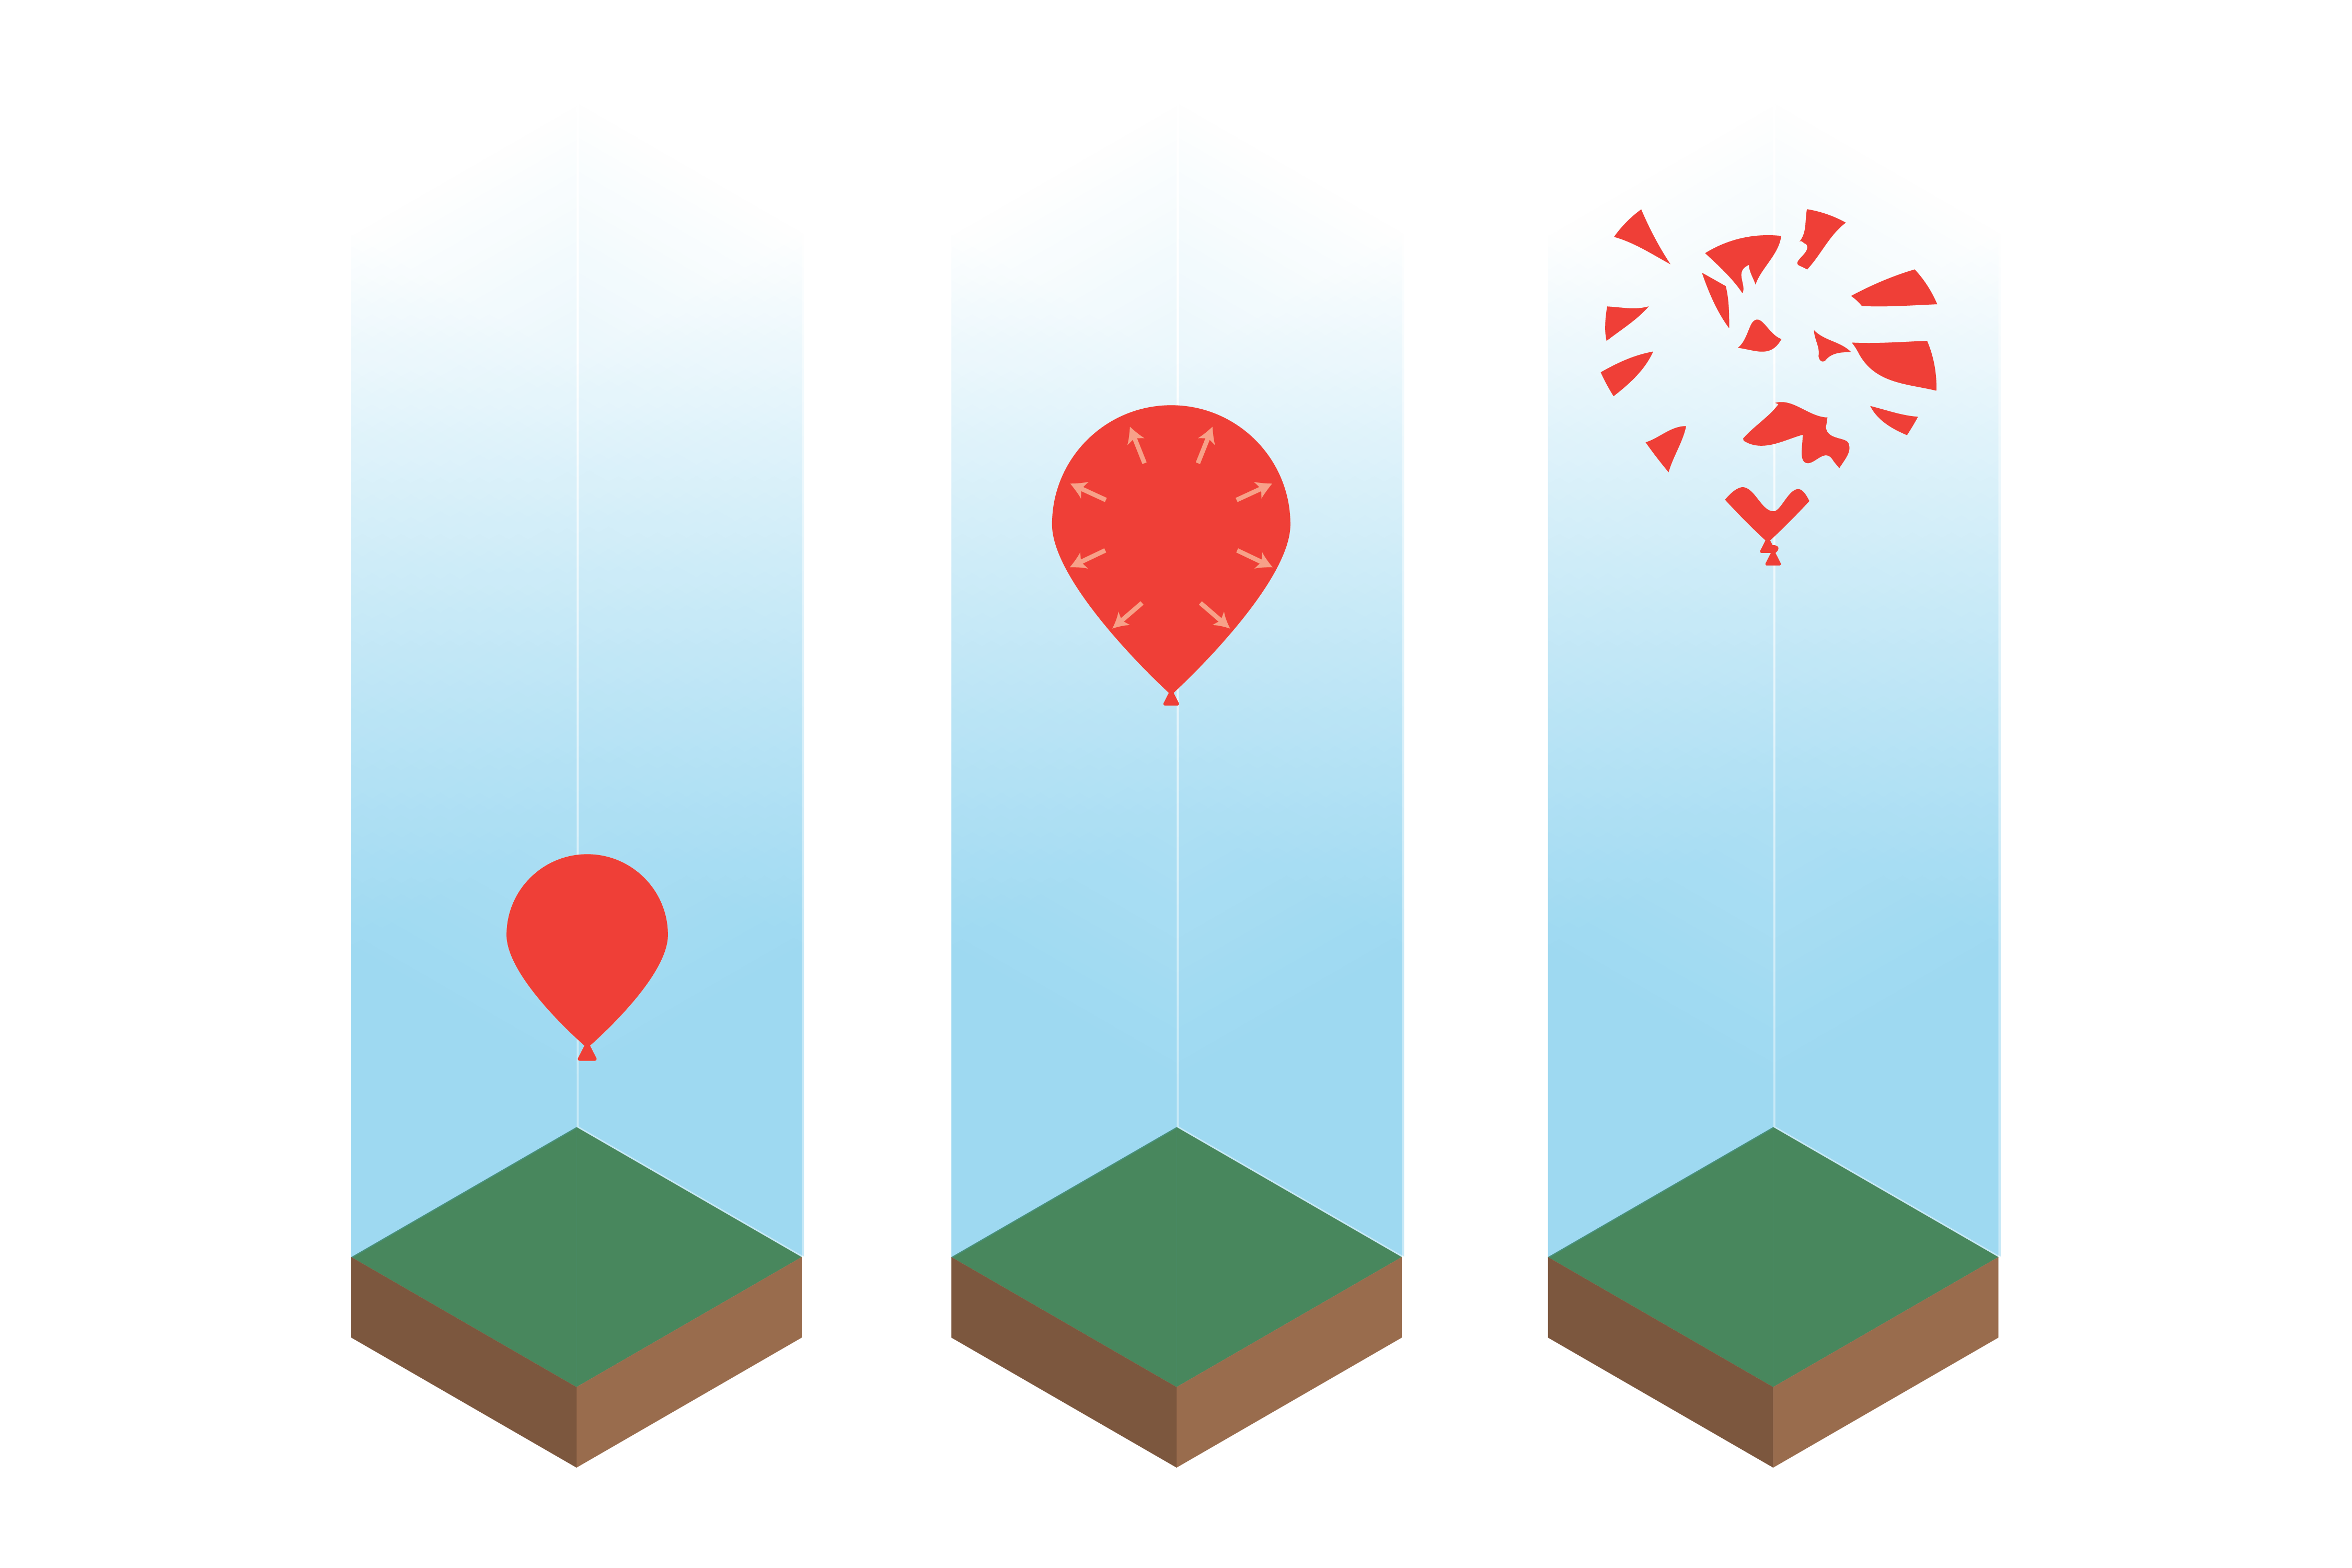
\includegraphics[width=\textwidth]{balloonColumn.png}

What would be the atmospheric pressure at $h$ meters above sea level?  Here is a handy formula for that:

$$p = 101,332 \times \left(1 - \left( 2.25577 \times 10^{-5} \times h\right) \right)^{5.25588}$$

where $p$ is the atmospheric pressure in pascals.

\begin{Exercise}[title={Atmospheric Pressure},  label=atmos_pressure]
  
You are thinking about riding your bicycle to the top of Mount Everest.  You are worried when the atmospheric pressure outside the tire drops,  the tire will fail.  
(I have had a tire fail before; It is very, very loud.)  

Calculate the atmospheric pressure at the top of Mount Everest (9,144 meters above sea level).

\end{Exercise}
\begin{Answer}[ref=atmos_pressure]

$$p = 101,332 \times \left(1 - 2.25577 \times 10^{-5} \times h\right)^{5.25588}$$

and $h = 9,144$.  Thus,

$$p \approx 30.1 \text{kPa}$$

\end{Answer}

\section{How a Straw Works}

\section{How Siphon Works}

\section{How a Toilet Works}
